\SetKw{State}{state}
\SetKw{Send}{send}
\SetKw{Wait}{wait}
\SetKw{Call}{call}
\SetKw{Return}{return}

\SetKwComment{Comment}{//}{}

\SetKwProg{Function}{function}{}{end}

\SetKwBlock{parallelblk}{Do In Parallel}{end}
\SetKwBlock{atomicblk}{atomic}{end}

\SetKwFunction{atomicAdd}{AtomicAdd}
\SetKwFunction{sortps}{sortByLamportEpoch}
\SetKwFunction{executeRetClie}{executeAndSubmitOpReply}
\SetKwFunction{clientSubmit}{Client::SubmitOp}
\SetKwFunction{leaderHandleAccept}{Leader::AcceptRespRecv}
\SetKwFunction{leaderHandleFinalAccept}{Leader::FinalAcceptRespRecv}
\SetKwFunction{clientWait}{Client::SubmitOpReplyRecv}
\SetKwFunction{Recover}{NewLeader::Recover}
\SetKwFunction{getPredecessor}{Leader::GetPredecessorTS}
\SetKwFunction{getSuccessor}{Leader::GetSuccessorTS}
\SetKwFunction{leaderSubmit}{Leader::SubmitOpRecv}
\SetKwFunction{replicaCoord}{Replica::coordRequestRecv}
\SetKwFunction{shardMain}{Leader::ProcessEpoch}
\SetKwFunction{leaderRecvCR}{Leader::SubmitCRRecv}
\SetKwFunction{CRReply}{Leader::SubmitCRRespRecv}
\SetKwFunction{append}{.append}
\SetKwFunction{find}{.find}
\SetKwFunction{pop}{.pop}
\SetKwFunction{adds}{.add}
\SetKwFunction{removes}{.remove}
\SetKwFunction{qpush}{.enq}
\SetKwFunction{qpop}{.deq}
\SetKwFunction{sorting}{.sort}
\SetKwFunction{clearing}{.clear}
\SetKwFunction{constructQueue}{constructQueue}
\SetKwFunction{execute}{execute}

\algnewcommand{\IfThenElse}[3]{% \IfThenElse{<if>}{<then>}{<else>}
  \algorithmicif\ #1\ \algorithmicthen\ #2\ \algorithmicelse\ #3}

\algnewcommand{\IfThen}[2]{% \IfThenElse{<if>}{<then>}{<else>}
  \algorithmicif\ #1\ \algorithmicthen\ #2}

\section{\sys{}}
\label{sec:design}
% 1. what are the key features it needs to do. which component of the protocol does that.
% 2. include parts in the motivation that describe why you can't simply do "X". and then in design you can refer to motivation...

\sys{} provides \mdl{} across shards with latency that approaches 1/4 that of Multi-Paxos, a \sdl{} protocol, as the number of concurrent client operations increases.
This section describes the design of \sys{} by
first giving a high-level overview of the protocol, why it provides \mdl{}, and why it provides lower latency.
Then we go over the details of \sys{}, including
its full protocol that decouples fault tolerance and ordering,
its special recovery protocol that runs when a shard leader fails,
and why it is correct.


\paragraph{\sys{} Overview.}
The key insight in \sys{} is to decouple fault-tolerance from ordering, allowing
parallelization of most processing of concurrent operations. To this end, the
\sys{} protocol has three phases for each set of concurrent operations from a
client: parallel replication for fault tolerance, sequential coordination, and
then parallel replication of ordering. The initial parallel replication occurs
before coordination and guarantees an operation is eventually executed.
This happening before coordination is what enables \sys{} to provide
suffix-closed failure semantics.  The sequential coordination ensures the legal
total order across shards and client issue order required by \mdl{} will exist.
Coordination is not replicated and requires only a single sequential
shard-to-shard message for each concurrent operation, which is what enables
\sys{} to provide lower latency.  Eliding replication for coordination is safe
because our recovery protocol allows us to safely redo coordination for
committed-but-not-ordered operations when leaders fail.  Finally,
replicating ordering in parallel ensures ordering information is durable before
execution.

\al{it would be nice to capture consicely here that the ordering before recovery
may be different after recovery, which is why we need to replicate ordering
before execution, but that that's ok but recovery ensures the order chosen will
respect all constraints on the total order}

% * provides mdl across shards\\
%* tolerates f crash failures per shard with 2f+1 replicas\\
%** each shard runs multi-paxos\\
%* does so with end-to-end app latency much lower that a similar sdl design: roughly 1/4 the latency\\


\subsection{Protocol}
This subsection details the \sys{} protocol.
It starts by going over the components and stepping through the protocol.
Then it discusses how the design achieves each of the following goals:
suffix-closed failure semantics,
\mdl{} ordering,
and lower latency.

\paragraph{Components and Protocol.}
\sys{} comprises two components: \textit{clients} that submit operations to a co-located \textit{client library} and \textit{shards} that store data and execute operations.
The client and shard protocols are shown in Algorithms~\ref{clientprotocol}, ~\ref{shardprotocolmessages}, and~\ref{shardprotocolcoord}.

\wl{should we say client-library maintains the set of outstanding operations and the predecessor id?\\
and the shards maintain a pending set, ordered log, and shard\_ts?}

The interface presented by the client library is a key-value store where arbitrary deterministic operations---e.g., read, write, read-modify-write---on a specified key are invoked immediately and return a future.
This asynchronous interface allows a client to dispatch many operations in parallel.

\todo{consider enumerating the steps here and shading which ones are on path or now}

When the client invokes an operation, the client library checks if there are any
outstanding operations.  The library sends the operation to the leader of the
appropriate shard along with a \textit{predecessor} id that identifies the most
recently-issued operation, or \textsc{null} if there is none.  In addition, when
there are outstanding operations, the client sends a coordination request
message to the shard leader for the predecessor operation that indicates this
operation as its \textit{successor}.

On receiving an operation's response from a shard leader, the client library buffers the operation until all prior operations are delivered to the application. We refer to this guarantee as \textit{return ordering}.

\wl{fix up shard leader vs server}

%% A key insight of \sys{} is to decouple fault-tolerance from ordering,
%% allowing replication of concurrent operations to proceed in parallel
%% on different shards, separate from ordering. While in existing
%% state-machine replication protocols operations are either uncommitted
%% or committed, operations in \sys{} proceed through the following four
%% states:

% \wl{``To do so, each shard shard maintains a \texttt{next\_ts} integer, initially zero, that is advanced whenever
% an operation is replicated and coordinated and at the end of each epoch. Upon arriving at a shard, an operation
% sets its tentative timestamp as the current value of \texttt{next\_ts}. An operation's timestamp is then
% finalized when it becomes coordinated and committed. Predecessors include their timestamps in their coordination
% responses. Successor operations then ensure that their timestamp is strictly greater than that
% of their predecessor. At the end of an epoch \texttt{next\_ts} is advanced to be strictly greater than the last
% operation in the epoch.''}

Operations at a shard go through four states:
\textit{pending},
\textit{committed},
\textit{coordinated},
and
\textit{ordered}.
When an operation first arrives at a shard leader, it is \textit{pending} and it is added to the set of pending operations.
The leader replicates the operation to its replicas, and once it receives a quorum of acknowledgements,
the operation is \textit{committed}.
Our protocol guarantees that a committed operation is eventually executed.
If this operation has a null predecessor it is immediately marked as \textit{coordinated}.
If this operation has a predecessor, then the leader waits until it receives the coordinate reply message from the predecessor to mark it as coordinated.
Once an operation is coordinated, it checks if it has received a coordination request, and if so immediately sends a coordination reply to the leader for \textit{its} successor operation.

Once an operation is marked coordinated the leader moves it from the pending set
into the next available instance in its ordered log.  It then replicates this
ordering to its replicas and, once it receives a quorum of acknowledgements, the
operation is \textit{ordered}.
The leader (and replicas) then execute operations in the order of the ordered log, i.e., an operation is executed as soon as it is ordered and the previous operation in the ordered log has been executed.

\todo{Mention ordering ack piggybacking parenthetically.}

Replication for each shard is done following the standard Multi-Paxos protocol, which tolerates $f$ crash failures with $2f+1$ replicas.
Updates to the pending set and ordered log are both replicated through Multi-Paxos.

When a leader receives a coordination request for an operation it has not yet coordinated (or received), it queues the request.
Conversely, when it receives a coordination request for an operation it already coordinated, it immediately sends the coordination reply message to the operation's successor.

\todo{Add a description of the first operation optimization here.}
\wl{can we apply this to all operations that arrive that are already coordinated? I think so!}

\paragraph{Suffix-closed Failures.}
\Mdl{} requires that if a client operation fails then all concurrent, but later issued operations fail.
\sys{} ensures such suffix-closed failures using coordinate replies that are only sent after an operation is committed and coordinated.
Ordering coordination replies after an operation is committed ensures the operation will be executed, either by the current leader in the normal case or by a new leader in the case of failover.
Ordering coordination replies after an operation is coordinated ensures this is transitively true for all of a client's earlier-issued concurrent operations.
For instance, if a client issues $o_1$, then $o_2$, then $o_3$, $o_3$ can only be coordinated after $o_2$ is coordinated, which can only be after $o_1$ is coordinated.
In turn, this means that $o_1$--$o_3$ were also committed and thus will eventually be executed.
Transitioning to the coordinated state is thus the point where an operation will eventually succeed.

Prior to this transition, an operation may fail for two reasons.
First, an operation will fail if it times out waiting for a coordination reply from its predecessor.
This can be triggered when the predecessor operation never arrives--e.g., the predecessor operation was dropped by the network and then the client machine failed so it cannot retransmit it.
Second, an operation will fail if it receives a special fail\_coordination reply instead of a success\_coordination reply.
In both cases, once an operation is failed the shard replies to the client with the failure.
In addition, the shard sends a fail\_coordination message to its successor operation if a coordination request is queued.
(If no coordination request is queued it tracks the failure so it can reply to a future coordination request with a fail\_coordination message.)


\paragraph{\Mdl{} Ordering.}
\Mdl{} requires a legal total order over all operations that respects real-time order and each client's issue order.
\sys{} ensures such an order exists through coordination messages that orchestrate the coordination and thus execution of operations around shards.

Execution on each shard is sequential, providing a legal total order for all operations on each shard.
That order respects real-time ordering constraints because of the normal guarantees of Multi-Paxos.
Relatedly, return ordering ensures real-time ordering 
constraints are consistent with each client's issue order: If a client's operation finishes and potentially introduces new real-time constraints, return ordering guarantees the client's prior operations (by issue order) already finished.

What is necessary then is to be able to show that the combination of all per-shard orderings and per-client issue ordering has a legal total order.
This is true if and only if the ordering constraints are acyclic.
The coordination messages ensure the constraints are acyclic by ensuring operations move to the coordinated state, and are thus added to each shard's ordered log, in their issue order.
This makes the two orders compatible: if $o_1$ is issue-ordered before $o_2$ by a client, then $o_1$ will be added to its shard's ordered log before $o_2$ is.

For example, consider a simple execution where client 1 issues $o_{a1}$ to shard A and then $o_{b2}$ to shard B and where client 2 issues $o_{b3}$ to shard B and then $o_{a4}$ to shard A.
Three out of four possible orderings of these operations are acyclic and thus \mdl{},
e.g., on shard A $o_{a1}$ then $o_{a4}$ and on shard B $o_{b3}$ then $o_{b2}$ is acyclic and thus there is a total order ($o_{a1}$,$o_{b3}$,$o_{b2}$,$o_{a4}$).
One of the four possible ordering creates a cycle and thus is not \mdl{}:
on shard A $o_{a4}$ then $o_{a1}$ and on shard B $o_{b2}$ then $o_{b3}$.
This interleaving creates a cycle where $o_{a4}$ is before $o_{a1}$ on shard A, $o_{a1}$ is before $o_{b2}$ by client 1's issue order, $o_{b2}$ is before $o_{b3}$ by shard B, and $o_{b3}$ is before $o_{a4}$ by client 2's issue order.
Our coordination messages preclude this cycle by controlling when operations are added to ordered logs.
In this case, they would ensure $o_{a4}$ is only added to the ordered log at shard A after $o_{b3}$ is added to the ordered log at shard B. In this example, this is after $o_{b2}$ is added to the ordered log, which in turn was only after $o_{a1}$ was added to the ordered log at shard A.

A complete proof that \sys{} provides \Mdl{} ordering is elided for brevity.

%\subsubsection{Operation vs.\@ End-To-End Latency}
\paragraph{Operation vs.\@ End-to-end Latency.}
Multi-Paxos provides \sdl{} with a single round of replication for both fault
tolerance and ordering.  \sys{}, in contrast, decouples replication for fault
tolerance and ordering into two rounds.  This increases the latency of
\textit{individual} operations but allows \sys{} to do each round of
replication for all of a client's concurrent operations in parallel. The only
sequential part of its protocol is the coordination messages.  The
coordination requests are sent by the client library and the coordination
replies are sent from shard to shard.  This puts at most a single shard-to-shard
message per operation in the sequential critical path of many concurrent client
operations. Moreover, these coordination messages may overlap with the first
round of replication.

The performance of both Multi-Paxos (assuming sequentially issued operations) and \sys{} depend on the number of concurrent client operations in the execution of an
application request as well as the number of distinct physical shards those
operations are sent to. Let $T$ be the one-way delay between machines (clients,
leaders, and replicas).  When there are $N$ (potentially) concurrent client
requests, Multi-Paxos's latency is $4*T*N$. On the other hand,
Figure~\ref{fig:mdlperf} shows \sys{} performance. Its latency
is $6T + (N-1)*T$ when each request lies at a different shard
than its predecessor.  Thus, while the latency of an individual operation is
higher in \sys{}, an application's end-to-end latency approaches
$1/4$ that of Multi-Paxos as the number of concurrent client requests grows.
% We
% specify worst case performance here since the coordination overhead for two
% consecutively issued concurrent requests that lay at the same shard is
% negligible, as it does not require a cross-shard message.}

%% As a result, a client's end-to-end application latency when using \sys{} scales by a factor
%% of the one-way cross-shard latency as the number of operations increases. In contrast,
%% the latency of applications using a \singledispatch{} system scales by a factor of the
%% quorum round-trip latency. Our evaluation in Section~\ref{sec:eval} bears out this claim.


%% \subsection{Client-Driven Coordination}

%% \sys{} shards coordinate with each other to ensure that operations are applied
%% according to the client's invocation order. But how do shards know which
%% operations are dependent on each other? One option would be for the client to
%% propagate dependencies along with each operation---each operation would include
%% the predeceeding concurrent requests that were invoked before it. However, this
%% would require an additional message from the shard responsible for an operation
%% and the shard of its predecessor to request coordination.

%% Instead, \sys{} introduces client-driven \textit{coordination requests (CR)},
%% that parallelize coordination requests with the operations themselves.  When a
%% client submits an operation to a shard, it also submits a CR, in parallel, to
%% the shard of its predecessor operation with the identity of the shard of its
%% successor.  In particular, for some operation issued by client $C$ with sequence
%% number $s$, a predecessor operation is defined as the concurrent operation that
%% client $C$ issued with sequence number $s-1$. If client $C$ does not have any
%% other outstanding operations, then the operation's predecessor is null.

%% Upon receiving a coordination request, a shard first waits until the operation
%% is committed and coordinated and then sends a \textit{coordination response} to
%% the shard leader of its successor. This inductively guarantees all of an
%% operation's predecessors will eventually succeed. An operation is considered
%% \textit{coordinated} if the shard has received a \textit{coordination response}
%% from the shard leader of the operation's predecessor.  (Operations without a
%% predecessor are vacuously coordinated.)




%% client-drive coordination makes the sequential coordination only take 1 shard-to-shard message.\\

%% \wl{I removed the 'respond to the client' claim about what happens after something is committed. That seem like an optimization only for write-only operations?}

%% \begin{figure}[!htb]
%% 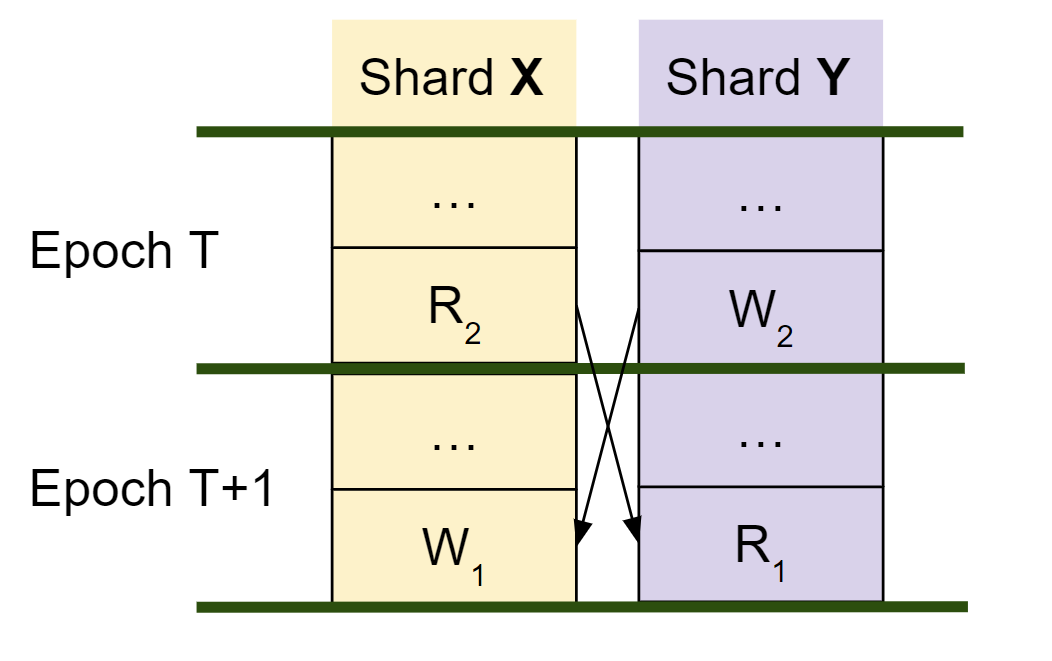
\includegraphics[scale=.3]{figs/sorted_batching_wrong.png}
%% \caption{Example execution of sorted batching without coordination requirement. This execution leads to an incorrect execution that contains a cycle and is not \mdl. The execution is the same execution as that of figure \ref{fig:concurrentbatches}, but now the second request issued by each client arrives in an earlier epoch. Even if sorted in their respective epochs, they are not ordered across epochs without coordination.}
%% \label{fig:sortedbatchingwrong}
%% \end{figure}

%% \subsection{Decoupling Fault-Tolerance \& Ordering}

%% Operations in a multi-shard system can fail independently, e.g., during leader
%% failure at one shard. Naively ordering a client's concurrent operations
%% independently at multiple shards, as many existing state-machine replication
%% protocols do, would violation \MDL{}'s invocation-order guarantee. On the other
%% hand, blocking operations on one shard on the completion of previously-invoked
%% operations on other shards in these systems would be impractically slow. The
%% problem is that existing state-machine replication protocols couple
%% fault-tolerance and ordering---e.g.\ leaders replicate both the operation itself
%% and its order in the log simultaneously. In order to guarantee suffix-closed
%% failure semantics, operations cannot be replicated until their predecessors have
%% also been replicated.

%The end-to-end latency of an application issuing $N$ operations to
%such a system would be approximately $N$ times one quorum round-trip plus one
%inter-shard message. This is worse than linearizable Raft, which just requires
%one quorum round-trip per operation.







%% \subsection{Lamport Timestamps For Issue Order}\label{sec:design:timestamps}

%% \wl{When is this timestamp assigned? I think it's exactly when an operation is 'coordinated'}

%% To ensure operations end up in a valid \MDL{} order, \sys{} assigns each operation a Lamport timestamp.
%% Operations are then sorted by their timestamp values (using arrival time at the shard to break ties)
%% at the end of an epoch.

%% Operations are assigned to maintain three invariants: (1) Each operation's timestamp must
%% be strictly greater than the timestamps of any operations that were previously replicated and coordinated
%% at the same shard; (2) an operation's timestamp is strictly greater than its predecessor's; and (3)
%% the timestamp of the first operation in each epoch is strictly greater than that of the last operation
%% in the previous epoch. 

%% To do so, each shard shard maintains a \texttt{next\_ts} integer, initially zero, that is advanced whenever
%% an operation is replicated and coordinated and at the end of each epoch. Upon arriving at a shard, an operation
%% sets its tentative timestamp as the current value of \texttt{next\_ts}. An operation's timestamp is then
%% finalized when it becomes coordinated and committed. Predecessors include their timestamps in their coordination
%% responses. Successor operations then ensure that their timestamp is strictly greater than that
%% of their predecessor. At the end of an epoch \texttt{next\_ts} is advanced to be strictly greater than the last
%% operation in the epoch.

%% TODO: Add intuition about why these invariants are needed.

% \md can only guarantee a safe total ordering across epochs of shards if it executes \textit{ordered} requests. Figure ~\ref{fig:sortedbatchingwrong} shows an execution that does not abide by this constraint, and only sorts committed (but not coordinated) requests within epochs. A cycle arises among all the requests across epoch boundaries, thus the execution does not have a total order and is not multi-dispatch linearizeable. A SUCCESS response for a given request's CR message, which coordinates it, serves as a promise that all predecessors have been sorted at the same or earlier epochs on their respective shards, which provides a total order across epochs of different shards.

% To to get invocation order, there are multiple mechanisms at play
% 1. sequence numbers
% 2. CR requests that are issued by clients
%       -these only get sent to the immediate predecessor (talk about inductive guarantees)
%       -these only get acked if all the other predecessors have been acked too, guaranteeing they are sorted as well. you can only be in an epoch equivalent to or greater than the epochs of your predecessors (not absolute values)

% Ensure that epcoh increase monotonically
% ensure that each epoch is executed in sorted order
% ensure that across epoch boundaries nothing fishy happens, guaranteed via CR acks
% ensure we have the extra round trip at the end to "order" commands (this is for failure too??)

% \subsection{Batching}
% \md makes use of batching to increase throughput and amortize the \textit{ordering} inter-replica round trip across multiple requests in an epoch. Multi-dispatch linearizeable back-end systems expect to experience more load than their single-dispatch linearizeable counterparts, since individual clients can issue many more requests in the former. For example, for $k$ shards, if clients submit on average 10 requests at a time, the logs at shards of \md backends will be about $10/k$ times longer than the logs of \sd shards. Thus batching is a nice way to handle processing of congested shard logs. Moreover, our coordination mechanism is independent across requests from different clients, thus we do not introduce any head-of-line blocking. For requests that arrive later but become coordinated sooner, those can be executed immediately without waiting on the coordination of requests from separate clients.
% Comment that we expect a more congested log at each shard since now there will be fanout from individual clients
% batching is a nice fit since it can exploit this high load
% moreover, ordering a request does not depend on previously arrived requests from independent clients to be ordered, hwich is a nice design that allows each client to see issue order scale with just their behavior, not other clients'.

\begin{comment}
\begin{figure}
\begin{tikzpicture}
[box/.style={draw=none, thick, font=\small, text centered, minimum height=1.2cm, minimum width=1.0cm}]
\newcommand\w{3}
\newcommand\h{5}

\node (clientbox) [box, yshift=6.5cm] {$C$};

\node (leaderbox) [box, yshift=6.5cm, xshift=\w cm] {$L_1$};

\node (replicabox) [box, yshift=6.5cm, xshift=2*\w cm] {$R$};
% C
\draw [stealth-](0,0) -- (0,\h+1);
% L1
\draw [stealth-](\w,0) -- (\w,\h+1);
% R1
\draw [stealth-](2*\w,0) -- (2*\w,\h+1);

% Left T{
\draw [decorate,
    decoration = {brace}] (\w-0.05,-0.15) --  (0,-0.15);
\node [box, yshift=-0.5cm, xshift=0.5*\w cm] {$T$};

% Right T{
\draw [decorate,
    decoration = {brace}] (2*\w,-0.15) --  (\w+0.05,-0.15);
\node [box, yshift=-0.5cm, xshift=1.5*\w cm] {$T$};


% Req1
\node [box, yshift=4.5cm, xshift=6.5cm] {$Req_1$};
% Top 4*T {
\draw [decorate,
    decoration = {brace}] (-0.15,4) --  (-0.15,5);
\node [box, yshift=4.5cm, xshift=-0.75 cm] {$4*T$};

% Req2
\node [box, yshift=3.25cm, xshift=6.5cm] {$Req_2$};
% Middle 4*T {
\draw [decorate,
    decoration = {brace}] (-0.15,2.75) --  (-0.15,3.75);
\node [box, yshift=3.25cm, xshift=-0.75 cm] {$4*T$};

% ReqN
\node [box, yshift=1.25cm, xshift=6.5cm] {$Req_N$};
% Bottom 4*T {
\draw [decorate,
    decoration = {brace}] (-0.15,0.75) --  (-0.15,1.75);
\node [box, yshift=1.25cm, xshift=-0.75 cm] {$4*T$};

% First request message < 4 Ts
\draw [-stealth](0,\h) -- (\w,0.95*\h);
\draw [-stealth](\w,0.95*\h) -- (2*\w,0.9*\h);
\draw [-stealth](2*\w,0.9*\h) -- (\w,0.85*\h);
\draw [-stealth](\w,0.85*\h) -- (0,0.8*\h);

% Second request messages < 8 Ts
\draw [-stealth](0,0.75*\h) -- (\w,0.7*\h);
\draw [-stealth](\w,0.7*\h) -- (2*\w,0.65*\h);
\draw [-stealth](2*\w,0.65*\h) -- (\w,0.6*\h);
\draw [-stealth](\w,0.6*\h) -- (0,0.55*\h);

% ellipses ...
\draw (0.2*\w,0.45*\h) node[auto=false]{\ldots};

% Last request message < 4*N Ts
\draw [-stealth](0,0.35*\h) -- (\w,0.3*\h);
\draw [-stealth](\w,0.3*\h) --  (2*\w,0.25*\h);
\draw [-stealth](2*\w,0.25*\h) -- (\w,0.2*\h);
\draw [-stealth](\w,0.2*\h) -- (0,0.15*\h);
\end{tikzpicture}
\caption{Performance for SDL. Since clients must issue requests sequentially, we expect N requests issued to take around $4*T*N$ units of time, where $T$ is the latency between servers. In our case we assume this latency is equivalent between clients and leaders, as well as leaders and replicas. We only display a single shard case since the latency should be equivalent for multiple shards.}
\label{fig:sdlperf}
\end{figure}
\end{comment}
%%%%%%%%%%%%%%%%%%%%%%%%%%%%%%%%%%%%%%%%%%%%%%%%%%%%%%
\begin{figure}
\begin{tikzpicture}
[box/.style={draw=none, thick, font=\small, text centered, minimum height=1.2cm, minimum width=1.0cm}]
\newcommand\w{0.8}
\newcommand\h{4.5}
\tikzset{snake it/.style={decorate, decoration=snake}}

\node (clientbox) [box, yshift=6cm] {$C$};

\node (leaderbox) [box, yshift=6cm, xshift=\w cm] {$L_1$};

\node (replicabox) [box, yshift=6cm, xshift=2*\w cm] {$R_1$};

\node (leaderbox) [box, yshift=6cm, xshift=3*\w cm] {$L_2$};

\node (replicabox) [box, yshift=6cm, xshift=4*\w cm] {$R_2$};

\node (leaderbox) [box, yshift=6cm, xshift=7*\w cm] {$L_N$};

\node (replicabox) [box, yshift=6cm, xshift=8*\w cm] {$R_N$};

% Client
\draw [stealth-](0,0) -- (0,\h+1);

% L1, R1
\draw [stealth-](\w,0) -- (\w,\h+1);
\draw [stealth-](2*\w,0) -- (2*\w,\h+1);

%L2, R2
\draw [stealth-](3*\w,0) -- (3*\w,\h+1);
\draw [stealth-](4*\w,0) -- (4*\w,\h+1);

%LN, RN
\draw [stealth-](7*\w,0) -- (7*\w,\h+1);
\draw [stealth-](8*\w,0) -- (8*\w,\h+1);

% Left T{
\draw [decorate,
    decoration = {brace}] (\w-0.05,-0.15) --  (0,-0.15);
\node [box, yshift=-0.5cm, xshift=0.5*\w cm] {$T$};

% Right T{
\draw [decorate,
    decoration = {brace}] (2*\w,-0.15) --  (\w+0.05,-0.15);
\node [box, yshift=-0.5cm, xshift=1.5*\w cm] {$T$};

% L2--LN T{
\draw [decorate,
    decoration = {brace}] (7.05*\w-0.05,-0.15) --  (3*\w,-0.15);
\node [box, yshift=-0.5cm, xshift=5*\w cm] {$T$};

% N request messages
\draw [-stealth](0,\h+0.6) -- node[midway,fill=white]{\footnotesize $R_1$}(\w,\h+0.2);
\draw [-stealth](0,\h+0.6) to[out=10, in=-200] node[midway,fill=white]{\footnotesize $R_2$} (3*\w,\h+0.2);
\draw [-stealth](0,\h+0.6) to[out=30, in=-200] node[midway,fill=white]{\footnotesize $R_N$} (7*\w,\h+0.2);

\draw [-stealth](0,\h+0.6) to[out=19, in=-190] (2.3*\w,\h+0.9);

% N paxos round trips
\draw [-stealth](\w,\h+0.2) -- (2*\w,\h-0.2);
\draw [-stealth](2*\w,\h-0.2) -- (\w,\h-0.6);

\draw [-stealth](3*\w,\h+0.2) -- (4*\w,\h-0.2);
\draw [-stealth](4*\w,\h-0.2) -- (3*\w,\h-0.6);

\draw [-stealth](7*\w,\h+0.2) -- (8*\w,\h-0.2);
\draw [-stealth](8*\w,\h-0.2) -- (7*\w,\h-0.6);

% First CR resp and client response
\draw[-stealth, dashed] (\w,\h-0.6) -- node[midway,fill=white]{\tiny $Coord_2$}(3*\w,\h-1);
\draw [-stealth](\w,\h-0.6) -- (0,\h-1);

% second CR resp and client response
\draw[-stealth, dashed] (3*\w,\h-1) -- node[midway,fill=white]{\tiny $Coord_2$}(5*\w,\h-1.4);
\draw [-stealth](3*\w,\h-1) -- (0,\h-1.4);

% Nth CR resp and client response
\draw[-stealth, dashed] (5*\w,\h-2.25) -- node[midway,fill=white]{\tiny $Coord_N$}(7*\w,\h-2.75);
\draw [-stealth](7*\w,\h-3.55) -- (0,\h-3.95);

% Ellipses
\draw (5*\w,\h-1.85) node[auto=false]{\ldots};
\draw (2.35*\w,\h+0.8) node[auto=false]{\ldots};
%Final Paxos round trip
\draw [-stealth](7*\w,\h-2.75) -- (8*\w,\h-3.15);
\draw [-stealth](8*\w,\h-3.15) -- (7*\w,\h-3.55);

% Brackets
\draw [decorate,
    decoration = {brace}] (-0.15,\h-0.57) --  (-0.15,\h+0.6);
\node [box, yshift=\h cm, xshift=-0.7 cm] {$3*T$};

\draw [decorate,
    decoration = {brace}] (-0.15,\h-2.75) --  (-0.15,\h-0.6);
\node [box, yshift=0.63*\h cm, xshift=-1.15 cm] {$(N-1)*T$};

\draw [decorate,
    decoration = {brace}] (-0.15,\h-3.95) --  (-0.15,\h-2.8);
\node [box, yshift=0.2*\h cm, xshift=-0.7 cm] {$3*T$};

% Horizontal lines
\draw[dashed] (0,\h+0.2) -- (8*\w,\h+0.2);
\draw[dashed] (0,\h-0.6) -- (8*\w,\h-0.6);
\draw[dashed] (0,\h-2.75) -- (8*\w,\h-2.75);


\end{tikzpicture}
\caption{Performance for MDL. Ommitted: Client issued coordination requests and final paxos ordering round trip for all requests except $R_N$ (shown). Since clients can issue multiple outstanding requests, we expect N requests to take around $6T + (N-1)*T$ units of time, where $T$ is the latency between servers and $N$ is the number of unique shards across all outstanding requests. In our case we assume this latency is equivalent between clients and leaders, leaders and replicas, as well as leaders to leaders.}
\label{fig:mdlperf}
\end{figure}
\todo{Unique shards is a weird way to put it, we only save on coordination request for consecutive requests to a single shard right?}

%% \subsection{Correctness}
%% We give a brief sketch of correctness for \protocol, showing why it guarantees \mdl. A more detailed discussion on leader failures follows in section ~\ref{subsec:leaderfailures}. We provide a full proof of correctness in our technical report ~\ref{}.

%% To guarantee \mdl, our protocol must provide a total order of operations that (1) respects per-client invocation order, (2) respects real time, and (3) respects our failure semantics. 

%% Our coordination request mechanism provides \md's failure semantics and also offers a vehicle to pass along lamport timestamps that can guarantee a safe linearization. Because requests coordinate their successors \textit{after} they themselves are coordinated and committed, the lamport timestamps they send include all causal relationships about requests ordered ahead of them in their log as well as requests invoked earlier by the same client. 
%% % Since shard leaders update their global timestamps immediately when requests are committed, coordinated, and added to the ordered log, the timestamps sent to successors also carry execution causal relationships within shards. 
%% Inductively, this ensures that all concurrent successors from the same client at possibly different shards carry these log and invocation orderings. Our coordination mechanism is also strong enough to provide real time guarantees.

%% Lastly, coordination requests provide our failure semantics by forwarding information about success and failures. If a request fails, all successors will either be notified of this failure and thus fail themselves and all successors, or, if not notified after a timeout period, they will pessimistically assume a failure and proceed to also fail themselves and their successors. This ensures a suffix closed set of failures, preceeded by a prefix closed set of successes.

%% \wl{Need to have said we told f failures with 2f+1 replicas by replicating each shard with multi-paxos earlier.}
%% \wl{Need to review the paxos rounds and state them somewhere, in particular replicas are accepting an operation into the ordered log at a given instance number}
%% \wl{Need to state we assume deterministic processing of operations, etc.}
%% \wl{Need to make the word choice for things the same everywhere (ordered log, execution log, ...)}

\subsection{Shard Leader Failover}
\label{subsec:leaderfailures}
Each shard is made fault tolerant to $f$ failures with $2f+1$ replicas running Multi-Paxos~\cite{lamport1998paxos}.
When a shard leader fails (or appears to fail), we call it the \textit{old leader}, and its replacement the \textit{new leader}.
Before processing any new operations the new leader runs a recovery protocol that allows us to safely (re)coordinate committed operations that have not been ordered.
This is what enables \sys{} to safely avoid replication being on-path between coordination replies, which keeps latency lower.

The recovery protocol first has the new leader ensure it has a complete, up-to-date ordered log as in typical Multi-Paxos:
it sends a request to the other replicas for entries in their ordered log,
once it has a quorum of replies it updates its ordered log to include any entries that other replicas have marked as accepted,
and then it finishes the protocol for those entries by sending accept messages to the replicas with them.\footnote{We elide details related to ballot numbers due to space constraints and because they are the same as in Multi-Paxos.}
This ensures that any ordered log entry the old leader could have executed and externalized will be in the new leader's ordered log.
An operation can only be executed after it is committed to the ordered log,
which only happens after it is accepted by a majority of replicas. In turn, this
ensures it will be seen and added to the ordered log of the new leader.

Ongoing operations can be in one of the four states: pending, committed, coordinated, or ordered.
Operations that are pending are equivalent to the network dropping the packet to the old leader and \stale{will be retried by the client}.
Operations that are ordered will be added to the ordered log of the new leader as discussed above.
This leaves operations that are committed and potentially also coordinated.
We do not replicate the coordination status of an operation to minimize the number of messages that are sequential for concurrent client requests.
Thus, we need to assume that any committed operation could have been coordinated.

This brings two requirements for recovering committed-but-not-ordered operations.
First, we must ensure they are executed to ensure suffix-closed failures.
%
Second, we must ensure all committed-but-not-ordered operations are ordered consistently with any potential previous ordering.
The first requirement is trivially satisfied by executing the operations in any order.
The second requirement is more complex and requires that we avoid introducing any cycles when considering shard ordering and client issue orderings.

%%%%%%%%%%%%%%%%%%%%%%%%%%%%%%%%%
%%%%%%%%% Client %%%%%%%%%%%%%%%%
%%%%%%%%%%%%%%%%%%%%%%%%%%%%%%%%%
\begin{algorithm}[!tb]
    \State $\textit{PID} \gets$ unique client ID\\
    \State $\mathcal{L} \gets \{...\}$ \algorithmiccomment{Shard Leaders}\\
    \State $\textit{seqno} \gets 0$, $\textit{rcvd} \gets 0$  \algorithmiccomment{Per Client}\\
    \State $\textit{prevReq} \gets \textit{NULL}$\\
    %\State $m$ \algorithmiccomment{mutex}\\
    \Function{\clientSubmit(\textit{Op}, K, V)}{
        $\textit{Req} := (\textit{Op}, K, V, \textit{PID}, \textit{seqno})$\\
        $\textit{seqno} = \textit{seqno} + 1$\\
        %$m.lock()$ \algorithmiccomment{Critical section begins}\\
        $\textit{prq} := \textit{prevReq}$\\
        $\textit{prevReq} \gets \textit{Req}$\\
        %$m.unlock()$ \algorithmiccomment{Critical section begins}\\
        \IfThen{$\textit{prevReq} \neq \textit{NULL}$}{\Send $\textit{SubmitCR}(\textit{prq}, \textit{Req})$ to $L_{K-1} \in \mathcal{L}$}\\
        \Send $\textit{SubmitOp}(\textit{Req})$ to $L_K \in \mathcal{L}$\\        
    }

    \Function{\clientWait(\textit{Req})}{
        \Wait receive $\textit{SubmitOpReply}(V)$ from $L_K \in \mathcal{L}$\\
        \Wait until $\textit{rcvd} = \textit{Req.seqno}$\\
        %$m.lock()$\\
        $\IfThen{\textit{prevReq} = \textit{Req}}{\textit{prevReq} \gets \textit{NULL}}$\\
        $\textit{rcvd} \gets \textit{rcvd} + 1$\\
        %$m.unlock()$\\
        \Return $V$\\
    }
    \caption{MD-Lin Client}
    \label{clientprotocol}
\end{algorithm}

%%%%%%%%%%%%%%%%%%%%%%%%%%%%%%%%%
%%%%% Shard Leader Communcation %
%%%%%%%%%%%%%%%%%%%%%%%%%%%%%%%%%
\begin{algorithm}[!tb]
    \Function{\leaderSubmit(\textit{Op}, K, V, P, s)}{
        % \If{$ClientSeqnoMap[P] \neq s$}{
        %     $buffer_{P}(\{Op, K, V, P, s\})$\\
        %     \algorithmiccomment{Buffer per-client out of order requests}\\
        %     \Return\\
        % }
        \algorithmiccomment{Issue this op}\\
        $\textit{bufferedMap}\append(\textit{Op}, K, V, P, s, 0)$\\
        % $ClientSeqnoMap[P]\mathrel{+}=1$\\
        \Send $\textit{Accept}(\textit{Op}, K, V, P, s)$ to all $r \in \mathcal{R}$\\
        % \For{$(Op, K, V, P, s) \in buffer_{P}$}{
        % \algorithmiccomment{Issue OoO buffered ops that are now ready}\\
        %     \If{$ClientSeqnoMap[P] = s$}{
        %         $bufferedMap\append{(Op, K, V, P, s, 0)}$\\
        %         $ClientSeqnoMap[P]\mathrel{+}=1$\\
        %         \Send $Accept(Op, K, V, P, s)$ to all $r \in \mathcal{R}$\\
        %     }
        % }
    }
    \Function{\leaderHandleAccept(\textit{req})}{
        $\textit{req.acks}\mathrel{+}=1$\\
        \If{$\textit{req.acks} \ge |Q|$} {
             $\textit{req.committed} \gets \textit{True}$\\
        }
        \If{$\textit{req.committed} \land \textit{req.coordinated}$}{
            $\textit{req.ts} := \max(\textit{req.ts}+1, \textit{ShardTS})$\\
            $\textit{ShardTS} := \max(\textit{req.ts}, \textit{ShardTS})+1$\\
            $\textit{SubmitCRResp}(\textit{req.succrq}, \textit{True}, \textit{req.ts})$ to $L_{K+1} \in \mathcal{L}$\\
            $\textit{bufferedMap}\pop(\textit{req})$\\
            $\textit{orderedLog}\append(\textit{req})$\\
            \Send $\textit{FinalAccept}(\textit{req})$ to all $r \in \mathcal{R}$\\            
        }
    }
    \Function{\leaderHandleFinalAccept(\textit{req})}{
        $\textit{req.facks}\mathrel{+}=1$\\
        \If{$\textit{req.facks} \ge |Q|$}{
            $v := \execute{req}$\\
            $\textit{SubmitOpReply}(\textit{req}, v)$ to $\textit{client}$\\
            \Send $\textit{Commit}(\textit{req})$ to all $r \in \mathcal{R}$\\
        }
    }   
    \caption{MD-Lin Shard Leader Communication}
    \label{shardprotocolmessages}
\end{algorithm}

%%%%%%%%%%%%%%%%%%%%%%%%%%%%%%%%%
%%%%%%%%% Failover %%%%%%%%%%%%%%
%%%%%%%%%%%%%%%%%%%%%%%%%%%%%%%%%
% getSuccessor(e)
% If e is in committed but not ordered
% BLOCK until I get my successor, then send back my_successor_ts -1
% Else if e in ordered 
% Return e.ts
% Else
% Return inf

\begin{algorithm}[!tb]
    \State $\textit{S}$ \algorithmiccomment{Set of all shards in cluster}\\
    \State $\textit{R}$ \algorithmiccomment{Set of all replicas in shard}\\
    % \State $n$ \algorithmiccomment{Number of replicas in shard}\\
    \textbf{parameter} $E$ \algorithmiccomment{Committed but not ordered ops}\\
    \Function{\Recover(\textit{E})}{\\
        \For{$\mathrm{each}$ $r \in R$}{ 
                \Wait receive $E_r$\\
                $E \gets E\cup E_r$\\
        }
        % $E \gets \bigcup\limits_{i=1}^{n} E_{i}$\\
        $\mathrm{init\_shard\_ts} \gets \mathrm{orderedLog}[-1].ts + 1$\\
        $\mathrm{shard\_ts} \gets \mathrm{init\_shard\_ts}$\\
        \For{$\mathrm{each}$ $ e \in E$}{
            \Send $\textit{getPredecessorTS}(e.\mathrm{pred})$ to $S_{e.\mathrm{pred}}$\\
            \Wait receive $\textit{getPredecessorTSReply}(ts)$ from $S_e$\\
            $e.\mathrm{pred\_ts} \gets ts$\\
            $e.\mathrm{succ\_ts} \gets \infty$\\
        }
        \For{$\mathrm{each}$ $s \in S$}{
            \Send $\textit{getSuccessor}(E)$ to $s$\\
            \Wait receive $\textit{getSuccessorReply}(TS)$ from $s$\\
            \For{$\mathrm{each}$ $ts_i \in TS$}{
                $e_i.\mathrm{succ\_ts} \gets \min(e_i.\mathrm{succ\_ts}, \enspace ts_i)$\\
            }
        }
        $E\sorting(\text{by} \enspace succ\_ts)$\\
        $q \gets \constructQueue(E)$\\
        \For{$e \in q$}{
            $e.\mathrm{ts} \gets \mathrrm{max}(e.\mathrm{pred\_ts}+1, \mathrm{shard\_ts})$\\
            $\mathrm{shard\_ts} \gets e.\mathrm{ts} + 1$\\
            $q\qpush(e)$\\
        }
        % $E\sorting(\text{by} \enspace arrival\_ts)$\\
        % $q \gets \constructQueue(E)$\\
        
        % % \For{$\mathrm{each}$ $e \in E$}{
        % %     $q\qpush(e)$\\
        % % }
        % \State $A \gets \{\}$\\
        % \State $C \gets \{\}$\\
        % \For{$e \in q$}{
        %     $e.\mathrm{ts} \gets \mathrrm{max}(e.\mathrm{pred\_ts}+1, \mathrm{shard\_ts})$\\
        %     $\mathrm{shard\_ts} \gets e.\mathrm{ts} + 1$\\
        %     \If{$e.\mathrm{ts} > e.\mathrm{succ\_ts}$}{
        %         $C\adds(e)$\\
        %     }
        %     \Else{
        %         $A\adds(e)$\\
        %     }
        %     $q\qpush(e)$\\
        % }
        % \While{$|C| > 0$}{
        %     \State $A\_tmp \gets \{\}$\\
        %     $q\clearing()$\\
        %     $C\sorting(\text{by} \enspace succ\_ts)$\\
        %     $\mathrm{shard\_ts} \gets \mathrm{orderedLog}[-1].ts + 1$\\
        %     \For{$\mathrm{each}$ $e \in C$}{
        %         $e.\mathrm{ts} \gets \mathrrm{max}(e.\mathrm{pred\_ts}+1, \mathrm{shard\_ts})$\\
        %         $\mathrm{shard\_ts} \gets e.\mathrm{ts} + 1$\\
        %         $q\qpush(e)$\\
        %         $A\_tmp\adds(e)$\\
        %     }
        %     $C\clearing()$\\
        %     \For{$\mathrm{each}$ $e \in A$}{
        %         $e.\mathrm{ts} \gets \mathrrm{max}(e.\mathrm{pred\_ts}+1, \mathrm{shard\_ts})$\\
        %         $\mathrm{shard\_ts} \gets e.\mathrm{ts} + 1$\\
        %         \If{$e.\mathrm{ts} > e.\mathrm{succ\_ts}$}{
        %             $C\adds(e)$\\
        %         }
        %         \Else{
        %             $A\_tmp\adds(e)$\\
        %         }
        %         $q\qpush(e)$\\
        %     }
        %     $A \gets A\_tmp$\\
        % }
        \Send $\textit{FinalAccept}(\textit{q})$ to all $r \in \mathcal{R}$\\
        \algorithmiccomment{New leader begins taking new client requests}
    }
    \Function{\getPredecessor(\textit{e})}{
        \Wait until $e.\mathrm{coordinated} \enspace \lor \enspace \textit{e} \in \mathrm{orderedLog}$\\
        \Return $e.\mathrm{ts}$\\
    }
    \Function{\getSuccessor(\textit{E})}{
        $V \gets$ constructEmptySet($|E|$)\\
        \For{$e_i \in E$}{
            \If{$\exists \enspace \textit{o} \notin \mathrm{orderedLog} \enspace \land \enspace o.\mathrm{committed} \enspace \land \enspace o.\mathrm{pred} = e$}{
                \Send $\textit{getSuccessor}(o)$ to all $S$\\
                \Wait receive $\textit{getSuccessorReply}(ts)$ from $S$\\
                $V_i \gets ts-1$\\
            }
            \If{$\exists \enspace \textit{o} \in \mathrm{orderedLog} \enspace \land \enspace o.\mathrm{pred} = e$}{
                $V_i \gets$ $o.\mathrm{ts}$\\
            }
            \Else{
                $V_i \gets$ $\infty$\\
            }
        }
        \Return $V$\\
    }
    \caption{MD-Lin Failover}
    \label{failover}
\end{algorithm}


\paragraph{Timestamps.}
To ensure a compatible ordering with other shards, the new leader issues coordination requests to the predecessors of all operations in the committed-but-not-ordered set.
These requests serve their aforementioned purpose and also return a predecessor timestamp, $ts_{pred}$, in the coordination reply. 

Once an operation is marked coordinated, in addition to ordering it in the log and replicating this order at a majority, the shard leader also assigns it a timestamp, ts, where $ts = \max(ts_{pred} + 1, ts_{leader})$ and $ts_{leader}$ is the leader's global timestamp. The shard leader also updates its global timestamp as $ts_{leader} = \max(ts_{leader}, ts_{op}) + 1$ after every operation that is marked coordinated and placed at an index in the log. An operation's timestamp is also replicated with the operation in the final ordering round to replicas.

Because we do not replicate the coordination status of an operation before sending a coordination response to its successor, new leaders must ensure that an operation's recovered timestamp is always compatible with any coordination responses sent by a prior leader. More specifically, an operation's timestamp must not increase compared to any previously assigned timestamp; otherwise, its timestamp may exceed its predecessor's.

To ensure this, during recovery, only an operation's predecessor timestamp is used to determine its timestamp.
(One more than the predecessor's is the minimum timestamp that could have been previously assigned to the operation.) 
Once all operations in the committed-but-not-ordered set are coordinated they are sorted by their timestamps, added to the ordered log, and replicated.
After all operations in that set have been replicated and thus moved to the ordered status, the new leader sets its shard timestamp and starts processing new operations from clients.

Since operations are assigned timestamps that are strictly greater than their predecessor, this protocol ensures the new leader executes recovered operations
in an order consistent with the clients' issue orders and the execution orders at other shards. If an operation $o_1$ is constrained to precede another operation $o_2$ through any combination of issue and per-shard ordering, $o_2$
is guaranteed to have a larger timestamp than $o_1$ by reasoning similar to that above during normal operation. 

% in a way similar to the normal coordination messages by ensuring their order is compatible with any other ordering on another shard.
% Consider two operations $o_m$ and $o_n$ on this shard where there is a path in the graph of constraints from $o_m$ to $o_n$.
% The recovery protocol ensures that $o_m$'s ts on the new leader, $\textit{ts}_\textit{m.new}$ is $\le$ its ts on the old leader, $\textit{ts}_\textit{m.old}$, because it is only based on the predecessor\_ts instead of the max of predecessor\_ts and shard\_ts.
% \stale{Further, if there is a path in the graph of constraints it can only go through coordinated operations that each ensure their ts is larger than both their predecessors and earlier operations on the same shard.
% Thus, the recovery protocol also ensures that $o_n$'s ts on the new leader, $\textit{ts}_\textit{n.new}$, is $>$ it's predecessor's ts, which by the transitive application of the timestamping rules is greater than $\textit{ts}_\textit{m.old}$.
% Together, this ensures that  $\textit{ts}_\textit{m.new}$ $\le$ $\textit{ts}_\textit{m.old}$ $<$ $\ldots$ $<$ $\textit{ts}_\textit{m.old}$ and thus the recovery protocol will compatibly order $o_m$ before $o_n$ when it sorts them based on the ts.}\footnote{Reasoning is similar, but significantly more complex, for cases where multiple shard leaders fail which we omit due to space constraints.}
% \wl{I dont really get this discussion clearly, will try to understand and rewrite if there is time.}

% \wl{The series of inequalities goes to m.old ... m.old, that must be a mistake, I think it should be n.old there but i dont see how that helps us}

%% special recovery can only change the shard ordering...
%% if there is a shard-ordering/issue-ordering path between A and B, then special recovery is guaranteed to order A before B:
%% if A and B were issued by the same client, then their sequence numbers cover this
%% if A and B were issued by different clients, then

%% A to A' shard ordered before B' to B

%% The ts of B will be based on the ts of B', which will have to be later than the ts of A'
%% A original ts is W
%% A' original ts is X > W (by ts\_new formula line)
%% B' original ts is Y > X (by ts\_new forumla)
%% B original ts is Z > Y > X > W

%% B new ts is J > Y > X > W
%% A new ts is K <= W (because it's picked to be based only on pred\_received\_ts and before it was a max that include that)
%% thus K <= W < X < Y < J ... K < J ... K will be executed first

%% (Also possible that multiple leader fail at the same time. That is also fine because the above reasoning precludes there being any inconsistent ordering with shard leaders that haven't failed. And for shard leaders that have failed, things will simply be executed in SOME pred\_received\_ts based order, which will only respect




%% Next, the recovery protocol identifies operations that have been committed-but-not-ordered.
%% Any ongoing operation is in one of the follwing intermediate states:
%% (1) arrived in the buffered map,
%% (2) committed,
%% (3) received a coordination response from its predecessor,
%% (4) been added to the execution log,
%% (5) coordinated its successor request,
%% (6) been committed in the execution log in this term,
%% (7) been executed, or
%% (8) responded to the client.
%% Operations in state 1 on the old leader are equivalent to the network dropping the pack to the old leader and will be retried by the client.
%% Operations in states 6--8 on the old leader will be added to the ordered log of the new leader as discussed above.
%% This leaves operations in states 2--5 to be recovery correctly.
%% The new leader can identify these operations by finding all committed operations that are not in its ordered log.

%


%% consider 4 operations:
%% clA: a1 b2
%% clB: b3 a4


%% a1 a4 and b2 b3 is good: a1, b2, b3, a4
%% a1 a4 and b3 b2 is good: a1, b3, b2, a4
%% a4 a1 and b3 b2 is good: b3, a4, a1, b2
%% a4 a1 and b2 b3 is bad: cycle from a4-a1-b2-b3-a4 so no total order

%% if a1 issue order before b2 AND b2 shard order before b3 THEN





%% \wl{WL pass through here}




%% These 



%% The interesting case to look at is a failure right after point (5). Any request $r$ that has already coordinated a successor request \textit{must} (A) be in the future logs of all leaders, to provide failure semantics, and (B) be placed in the correct order in the log post-failure, to guarantee invocation ordering. These guarantees are less important for requests that have not coordinated a successor since those requests have no impact on successors that might externalize this state, and clients can simply reissue these requests if they fail/are lost.

%% \wl{Drop the whole sentence what says ``these guarantees are less...'', we don't know which ones those are so we have to safely handle all of these}

%% To guarantee (A), after an election completes, any new leader must ask for the buffered logs of at least a quorum of replicas to ensure it has every request that might have successfully coordinated a successor requests. We do not replicate the coordination bit on non-leader nodes, since this would diminish our opportunity to parallelize coordinating an entry and making it fault tolerant. By extension, knowledge of which requests have coordinated their successors only exists at the leader, this information is also not replicated. Because of this, there is no way for a new leader to know which buffered entries are coordinated themselves or have coordinated successor requests, so it performs this log diff. This technique is similar to View-Stamped Replication's ~\ref{} \texttt{DoViewChange} messages sent from replicas to leaders during a view change. 

%% Crucially, if this step is omitted, a leader might be elected that is missing an entry that coordinated a successor request. For example, consider a network partition which creates two subclusters, each of which contains a node operating as a leader (one in a later term than the other). The subcluster that contains a quorum could receive a request and in the future coordinate its successor at another shard after it itself has been committed and coordinated. Consider when the leader of this subcluster fails to deliver the commit messages to replicas to order this entry at this log index, and immediately afterwards the partition is removed. At this point, no replica that might become a leader is aware of the fact this entry has coordinated its successor, or even that it has moved from the buffered map and to the ordered log. There is no available information among the replicas to reconstruct this information, so we must pessimistically assume all buffered entries at a quorum of nodes have coordinated their successors and include them in the buffered log of the newly elected leader.

%% To provide (B), at the beginning of each new term, a newly elected leader must immediately process all buffered entries and place them in the ordered log before accepting any future client requests (or fail them if their predecessors failed). This is an expensive task during which the new leader must reissue each buffered request's coordination message (that the client sent initially) to the predecessor shard and wait for a response. In parallel, the new leader must also replicate each buffered request at a new quorum of nodes to ensure the entry exists on a quorum of replicas across multiple leader failures (the buffered log is not persisted).

%% \wl{make it clear, we are failing *operations* if the predecessor *operation* failed.}

%% As the new buffered entries at the new leader become committed and coordinated, we do not immediately add them to the ordered log. Moreover, we do not update the global shard timestamp between each commit/coordination event. Finally, once the last buffered entry is committed and coordinated, we enter all entries in sorted timestamp order to the ordered log (or fail them if their predecessor failed). Without this expensive buffer flushing, it is possible that a new request $r'$ might arrive and become committed and coordinated before a buffered entry $r$ that was committed and coordinated at the previous leader is committed and coordinated with the current leader. Linearizability could be violated if $r'$ must be ordered in the log after $r$ but is placed in the ordered log before $r$. The lamport timestamps guarantee a safe total ordering that respect any causal relationships. While we might reorder operations that are not causally related, this is safe and does not violate \mdl. 

%% Finally, we mention that coordination requests might also be lost in the network or across leader failures. To solve this, each request has a fixed amount of total epochs for which it can remain uncoordinated. After a leader sees that a request is "stale", it will fail the request as well as any pending coordination requests from successors of that request, beginning the suffix closed failure set. This solution also handles the garbage collection of the buffered log.







%% To begin, we employ a similar voting mechanism as Raft for selecting the leader from the candidate from the highest term that has the most up-to-date log, where in this case the log is the ordered log of requests that were sorted and executed in prior epochs. This ensures that all committed and executed (and possibly client-externalized) requests are in all future leader logs. Next we describe how buffered requests are safely carried across successive terms with different leaders.

%% \wl{need to update, ``all committ/executed requests will be in all future leader logs'' is incorrect. Because we don't use the consistency check from RAFT, you can have a 3-replica system where you have a L and R1 and R2. L tells R1 about committed and executed op1 and it tells R2 about committed and executed op2. Neither R1 nor R2 have all committed requests}

%% During operation of \protocol, requests can exist in multiple intermediate states. Specifically, a failure could occur after a request has (1) arrived in the buffered map, (2) been committed, (3) received a coordination response from its predecessor, (4) been added to the execution log (5) coordinated its successor request, (6) been committed in the execution log in this term, (7) been executed, or (8) responded to the client. 

%% \wl{failure between 1 and 2 is like the client's request packet being dropped, failure after 6 is safe because the new leader will reexecute the operation, but get the same result (by the definition of RSMs), and the client will get a redundant response it will drop. this leave failure after 2 and before 6, which all look the same and thus need to be handled the same. What is necessary for operations in this in-between period is ...}

%% The interesting case to look at is a failure right after point (5). Any request $r$ that has already coordinated a successor request \textit{must} (A) be in the future logs of all leaders, to provide failure semantics, and (B) be placed in the correct order in the log post-failure, to guarantee invocation ordering. These guarantees are less important for requests that have not coordinated a successor since those requests have no impact on successors that might externalize this state, and clients can simply reissue these requests if they fail/are lost.

%% \wl{Drop the whole sentence what says ``these guarantees are less...'', we don't know which ones those are so we have to safely handle all of these}

%% To guarantee (A), after an election completes, any new leader must ask for the buffered logs of at least a quorum of replicas to ensure it has every request that might have successfully coordinated a successor requests. We do not replicate the coordination bit on non-leader nodes, since this would diminish our opportunity to parallelize coordinating an entry and making it fault tolerant. By extension, knowledge of which requests have coordinated their successors only exists at the leader, this information is also not replicated. Because of this, there is no way for a new leader to know which buffered entries are coordinated themselves or have coordinated successor requests, so it performs this log diff. This technique is similar to View-Stamped Replication's ~\ref{} \texttt{DoViewChange} messages sent from replicas to leaders during a view change. 

%% Crucially, if this step is omitted, a leader might be elected that is missing an entry that coordinated a successor request. For example, consider a network partition which creates two subclusters, each of which contains a node operating as a leader (one in a later term than the other). The subcluster that contains a quorum could receive a request and in the future coordinate its successor at another shard after it itself has been committed and coordinated. Consider when the leader of this subcluster fails to deliver the commit messages to replicas to order this entry at this log index, and immediately afterwards the partition is removed. At this point, no replica that might become a leader is aware of the fact this entry has coordinated its successor, or even that it has moved from the buffered map and to the ordered log. There is no available information among the replicas to reconstruct this information, so we must pessimistically assume all buffered entries at a quorum of nodes have coordinated their successors and include them in the buffered log of the newly elected leader.

%% To provide (B), at the beginning of each new term, a newly elected leader must immediately process all buffered entries and place them in the ordered log before accepting any future client requests (or fail them if their predecessors failed). This is an expensive task during which the new leader must reissue each buffered request's coordination message (that the client sent initially) to the predecessor shard and wait for a response. In parallel, the new leader must also replicate each buffered request at a new quorum of nodes to ensure the entry exists on a quorum of replicas across multiple leader failures (the buffered log is not persisted).

%% \wl{make it clear, we are failing *operations* if the predecessor *operation* failed.}

%% As the new buffered entries at the new leader become committed and coordinated, we do not immediately add them to the ordered log. Moreover, we do not update the global shard timestamp between each commit/coordination event. Finally, once the last buffered entry is committed and coordinated, we enter all entries in sorted timestamp order to the ordered log (or fail them if their predecessor failed). Without this expensive buffer flushing, it is possible that a new request $r'$ might arrive and become committed and coordinated before a buffered entry $r$ that was committed and coordinated at the previous leader is committed and coordinated with the current leader. Linearizability could be violated if $r'$ must be ordered in the log after $r$ but is placed in the ordered log before $r$. The lamport timestamps guarantee a safe total ordering that respect any causal relationships. While we might reorder operations that are not causally related, this is safe and does not violate \mdl. 

%% Finally, we mention that coordination requests might also be lost in the network or across leader failures. To solve this, each request has a fixed amount of total epochs for which it can remain uncoordinated. After a leader sees that a request is "stale", it will fail the request as well as any pending coordination requests from successors of that request, beginning the suffix closed failure set. This solution also handles the garbage collection of the buffered log.

%%%%%%%%%%%%%%%%%%%%%%%%%%%%%%%%%
%%%%% Shard Leader Coordination %
%%%%%%%%%%%%%%%%%%%%%%%%%%%%%%%%%
% \begin{algorithm}
%     \State $ShardTS \gets 0$\\
%     \State $Timer \gets T$\\
%     \State $accepting \gets True$\\
%     \State $bufferedMap \gets []$\\
%     \State $orderedLog \gets []$\\
%     \State $ClientSeqnoMap \gets [][]$\\
%     \Function{\shardMain{}}{
%         \Wait until $Timer = 0$\\
%         $accepting \gets False$\\
%         $batch := []$\\
%         \For{$entry \in bufferedMap$\\}{
%             $entry.epochsSeen\mathrel{+}=1$\\
%             \If{$entry.committed \land entry.coordinated$\\}{
%                 %$entry.epoch \gets ShardTS$\\
%                 $batch\append{entry}$\\
%                 $ShardTS = Math.max(ShardTS, entry.epoch)$\\
%                 $bufferedMap\pop(entry)$\\
%             }
%             \ElseIf{$entry.epochsSeen > MAX\_EPOCHS$}{
%                 $bufferedMap\pop(entry)$\\
%                 $SubmitCRResp(entry, False)$ to $L_{K+1} \in \mathcal{L}$\\
%             }
%         }
%         \sortps{batch}\\
%         $orderedLog\append{batch}$\\
%         $ShardTS \mathrel{+}=1$\\
%         \Send $FinalAppendEntries(batch)$ to all $r \in \mathcal{R}$\\
%         %\Wait receive $AppendEntriesSuccess$ from all $r \in Q \in \mathcal{R}$\\
%         %$bufferedMap\popO{}$\\
%         $\executeRetClie{batch}$\\
%         %$\atomicAdd(ShardTS, 1)$\\
%         $accepting \gets True$\\
%         $Timer \gets T$\\
%     }
%     \caption{MD-Lin Shard Leader Epoch Handling}
%     \label{shardprotocolmain}
% \end{algorithm}

\begin{algorithm}[!tb]
    \Function{\leaderRecvCR(\textit{rq}, \textit{succrq})}{
    \algorithmiccomment{Received CR from client of succrq}\\
        $\textit{rq.succrq} := \textit{succrq}$\\
        \If{$\textit{entry} := \textit{orderedLog}\find(\textit{rq}) \neq \textit{NULL}$}{
            $\textit{SubmitCRResp}(\textit{succrq}, \textit{True}, \textit{entry.ts})$ to $L_{K+1} \in \mathcal{L}$\\
            \Return\\
        }
        \Wait $\textit{entry} := \textit{bufferedMap}\find(\textit{rq}) \neq \textit{NULL}$\\
        \Wait $(\textit{entry.committed} \land \textit{entry.coordinated}) \lor \textit{bufferedMap}\find(\textit{rq}) = \textit{NULL}$\\
        \If{$\textit{entry.committed} \land \textit{entry.coordinated}$}{
            $\textit{SubmitCRResp}(\textit{succrq}, \textit{True}, \textit{entry.ts})$ to $L_{K+1} \in \mathcal{L}$\\
        }
        \Else{
            $\textit{SubmitCRResp}(\textit{succrq}, \textit{False}, -1)$ to $L_{K+1} \in \mathcal{L}$\\
        }        
    }
    \Function{\CRReply(\textit{req}, v, \textit{ts})}{
        
        \If{$v = \textit{True}$}{
            % \Wait $entry := bufferedMap\find{rq} \neq NULL$\\
            $\textit{req.coordinated} \gets \textit{True}$\\
            $\textit{req.ts} = \textit{ts}$\\
            \If{$\textit{req.committed} \land \textit{req.coordinated}$}{
                $\textit{req.ts} := \max(\textit{req.ts}+1, \textit{ShardTS})$\\
                $\textit{ShardTS} := \max(\textit{req.ts}, \textit{ShardTS})+1$\\
                $\textit{SubmitCRResp}(\textit{req.succrq}, \textit{True}, \textit{req.ts})$ to $L_{K+1} \in \mathcal{L}$\\
                $\textit{bufferedMap}\pop(\textit{req})$\\
                $\textit{orderedLog}\append(\textit{req})$\\
                \Send $\textit{FinalAccept}(\textit{req})$ to all $r \in \mathcal{R}$\\            
            }
        }
        \Else{
            $\textit{bufferedMap}\pop(\textit{rq})$\\
            $\textit{SubmitCRResp}(\textit{rq.succrq}, \textit{False}, -1)$ to $L_{K+1} \in \mathcal{L}$\\
        }
    
    }
    \caption{MD-Lin Shard Leader Coordination}
    \label{shardprotocolcoord}
\end{algorithm}
\wl{The algorithms need to wrap words in textit to get proper kerning, e.g., $buffered$ vs $\textit{buffered}$}

